\chapter{Results and Discussion}
\label{ch:results_and_discussion}

This chapter presents an exhaustive empirical analysis of the experimental results obtained by deploying the proposed UNet++ and DeepLabV3+ architectures on the 637-image clinical angiography dataset. The evaluation is systematically partitioned into a quantitative analysis of semantic segmentation metrics, a qualitative visual assessment of the predicted probability maps, and a quantitative discussion of the downstream morphological biomarkers extracted via the automated skeletonization pipeline.

\section{Quantitative Semantic Segmentation Results}
The fundamental objective of the primary deep learning phase is to maximize the spatial overlap between the predicted binary vessel masks and the expert-annotated ground truth. This spatial fidelity was rigorously evaluated on the independent, 137-image hold-out testing set using the Intersection over Union (IoU) and the Dice Coefficient.

\subsection{Convergence and Learning Dynamics}
The training of all models was governed by the hybrid Binary Cross-Entropy and Dice Loss ($\mathcal{L}_{BCE+Dice}$) formulation. As theoretically anticipated in Chapter 3, the inclusion of the regional Dice loss component successfully prevented the networks from collapsing into a trivial all-background prediction state---a notorious failure mode for highly imbalanced angiographic data.

Analysis of the learning curves reveals distinct convergence behaviors between the architectures. The \textbf{DeepLabV3+} architecture, leveraging its ImageNet-pretrained ResNet50 backbone, demonstrated remarkably rapid early convergence. Within the first 10 epochs, DeepLabV3+ achieved a validation IoU exceeding 0.84. However, the performance plateaued shortly thereafter, triggering the \texttt{ReduceLROnPlateau} scheduler to decay the learning rate from $1 \times 10^{-4}$ to $2 \times 10^{-5}$. The model ultimately converged at epoch 14, where the \texttt{EarlyStopping} callback terminated training to prevent overfitting, restoring the optimal weights from epoch 13 which yielded a validation loss of $0.4714$.

Conversely, the \textbf{UNet++ (Scratch)} architecture exhibited a much slower, yet highly stable, initial learning phase. Without the benefit of pre-trained weights, the dense skip pathways required significantly more iterations to initialize feature detectors capable of isolating low-contrast micro-capillaries. However, the \textbf{UNet++ (ResNet50)} variant combined the rapid early convergence of the pre-trained backbone with the deep feature aggregation of the dense decoder, resulting in the most stable overall learning trajectory with the lowest variance in validation loss across the final 15 epochs.

\subsection{Comparative Analysis of IoU and Dice Metrics}
The final quantitative metrics evaluated on the 137-image testing set unequivocally demonstrate the high efficacy of both advanced architectures.

\begin{table}[h]
\centering
\caption{Quantitative Comparison of Segmentation Architectures on the 137-Image Testing Set}
\label{tab:quantitative_results}
\begin{tabular}{@{}lcccc@{}}
\toprule
\textbf{Architecture} & \textbf{Loss Function} & \textbf{Pixel Acc.} & \textbf{Val. IoU} & \textbf{Val. Dice} \\ \midrule
UNet (Baseline) & BCE & 0.9412 & 0.7645 & 0.8665 \\
UNet++ (Scratch) & BCE + Dice & 0.9588 & 0.8210 & 0.9017 \\
UNet++ (ResNet50) & BCE + Dice & \textbf{0.9631} & \textbf{0.8605} & \textbf{0.9250} \\
DeepLabV3+ & BCE + Dice & 0.9590 & 0.8547 & 0.9216 \\ \bottomrule
\end{tabular}
\end{table}

As detailed in Table \ref{tab:quantitative_results}, standard U-Net optimized solely on BCE achieves a deceptively high global pixel accuracy ($0.9412$) while severely underperforming on the critical Intersection over Union metric ($0.7645$). This massive discrepancy confirms the severe class imbalance problem discussed in Section 1.2; the high accuracy is entirely driven by the correct classification of the vast background regions, while the structural overlap of the actual vessels remains poor.

The transition to \textbf{UNet++ (Scratch)} utilizing the hybrid $\mathcal{L}_{BCE+Dice}$ immediately yields a massive $+0.0565$ absolute improvement in Validation IoU. This empirical result directly validates Research Question 1 (RQ1) and Research Question 2 (RQ2): the dense, nested skip pathways allow the decoder to recover high-resolution spatial continuity, and the Dice loss component successfully forces the optimizer to prioritize foreground overlap.

Both pre-trained architectures perform exceptionally well. \textbf{DeepLabV3+} achieves a stellar Validation IoU of $0.8547$ and a Validation Dice of $0.9216$. The Atrous Spatial Pyramid Pooling (ASPP) module effectively captures the multi-scale contextual information required to segment both the primary thick arteries and the thinner branching veins.

However, the highest overall performance is achieved by \textbf{UNet++ (ResNet50)}, peaking at a Validation IoU of $0.8605$ and a Dice Coefficient of $0.9250$. The empirical evidence suggests that while DeepLabV3+'s ASPP is highly effective, the dense semantic aggregation occurring across the $X_{i,j}$ grid of UNet++ provides a slight, but measurable, advantage in preserving the absolute finest, single-pixel-wide micro-capillaries at the extreme periphery of the angiograms.

\section{Qualitative Visual Assessment}
While numerical metrics like IoU provide a global statistical summary, the clinical utility of a segmentation model is ultimately judged by the visual continuity and structural integrity of the predicted probability maps. Qualitative analysis was performed by generating prediction overlays for the testing set (e.g., \texttt{overlay\_501\_RGB.jpg.png} through \texttt{overlay\_510\_RGB.jpg.png}).

\subsection{Resolution of Thick vs. Thin Vessels}
Visual inspection of the DeepLabV3+ prediction overlays confirms the numerical data. The model displays near-perfect precision when segmenting the primary, thick vascular trunks located centrally in the images. The boundaries of these thick vessels are predicted with exceptionally high probability ($P \rightarrow 1.0$), resulting in sharp, smooth edges devoid of jagged artifacts.

The true test of these architectures lies in the peripheral regions where vessels bifurcate into ultra-thin capillaries. Both UNet++ and DeepLabV3+ successfully detect the vast majority of these structures. However, qualitative differences emerge at the absolute resolution limits (vessels $\le 2$ pixels wide). DeepLabV3+ occasionally exhibits fragmentation; it correctly identifies the presence of the capillary but predicts a discontinuous, dashed line. This fragmentation occurs because the spatial down-sampling in the encoder (even with atrous convolutions) fundamentally loses some spatial information that the single up-sampling pass in the decoder struggles to fully reconstruct.

In contrast, the dense skip connections of UNet++ demonstrate superior performance in maintaining the continuity of these ultra-thin structures. By constantly shuttling high-resolution spatial features directly from the early encoder layers to the final decoder block, UNet++ bridges the spatial gaps that cause fragmentation in DeepLabV3+. 

\subsection{Handling Pathological Noise and Low Contrast}
Both models demonstrated excellent robustness against uneven background illumination, a direct consequence of the aggressive brightness and contrast augmentation applied via Albumentations during training. In regions where the contrast agent density drops significantly, causing the vessel to visually fade into the tissue background, the models correctly leverage the broader contextual layout (the direction and curvature of the vessel leading into the low-contrast zone) to infer the presence of the vessel, resulting in continuous segmentations where traditional thresholding would inevitably fail.

\section{Morphological Topological Biomarkers (Skeletonization)}
The culmination of this thesis pipeline is the automated extraction of quantitative morphological biomarkers from the raw pixel segmentations. This is achieved through the downstream application of mathematical skeletonization algorithms to the binary masks predicted by the deep learning models.

\subsection{Extraction of Distinct Vessel Networks}
Following the binarization of the probability maps, the Zhang-Suen thinning algorithm reduces the complex, varying-width vascular tree into a strictly 1-pixel wide topological skeleton. By running a Connected Component Labeling algorithm on this skeleton, the system autonomously counts the number of distinct, structurally isolated vascular networks present in the angiogram.

Analysis of the generated \texttt{vessel\_counts.csv} report for the testing set reveals highly consistent biological structures. For example, Image ID 501 yielded 15 distinct connected networks, Image ID 502 yielded 19 networks, and Image ID 506 yielded 12 networks. Across a random sample of 10 test images (IDs 501-510), the pipeline detected an average of $15.9$ distinct networks per image. 

The variation in the number of distinct networks provides immediate clinical insight. A significantly elevated count of distinct networks in a single localized region could be a strong indicator of pathological neovascularization (the uncontrolled proliferation of fragile new blood vessels, a hallmark of severe Diabetic Retinopathy). Conversely, a severely reduced network count might indicate localized ischemia or vascular occlusion. By automating this count, the proposed pipeline transitions from a simple image processing tool to a diagnostic assistant.

\subsection{Branch Points and End Points}
The skeletonization pipeline further analyzes the connectivity of the 1-pixel thick graph to identify critical topological nodes: branch points (bifurcations) and end points (terminations). 

The \texttt{vessel\_counts.csv} data highlights the extreme density of the vascular network. Image ID 501 contains 3,211 distinct branch points, while Image ID 506 contains 3,640 branch points. The ratio of branch points to end points (e.g., 3,211 branch points to 59 end points in Image 501) numerically describes the extreme interconnectivity and looping nature of the vascular tree. 

These massive, precise nodal counts are physically impossible for a human clinician to extract manually. The ability of the proposed UNet++/DeepLabV3+ pipeline to first cleanly segment the network, and the subsequent skeletonization algorithm to autonomously extract thousands of precise topological nodes in mere seconds, definitively answers Research Question 3 (RQ3) and establishes the high clinical value of the integrated methodology.

\section{Egg Embryo Vessel Growth Analysis}
The primary biological application of the developed deep learning and skeletonization pipeline is to perform a quantitative comparative analysis of angiogenesis kinetics in egg embryos. We evaluated vascular growth over time (0h, 2h, 4h, 8h, 24h, 32h) when exposed to varying concentrations of a therapeutic agent (Control, 0.1\,$\mu$g, 1\,$\mu$g, and 10\,$\mu$g).

By matching the 637 cropped images back to their raw dataset folders using downscaled Mean Squared Error (MSE) matching, each image was successfully assigned its concentration and timepoint metadata. The trained UNet++ model segmented the vascular networks, and the morphological thinning pipeline extracted three primary topological metrics: Vessel Networks, Branch Points, and End Points. The aggregated statistics are detailed in Table~\ref{tab:egg_embryo_growth}.

\begin{table}[htbp]
\centering
\caption{Quantitative Morphological Metrics of Egg Embryo Angiogenesis over Time}
\label{tab:egg_embryo_growth}
\small
\begin{tabular}{lccccc}
\toprule
\textbf{Concentration} & \textbf{Time Point} & \textbf{n} & \textbf{Networks (Mean $\pm$ SD)} & \textbf{Branch Points (Mean $\pm$ SD)} & \textbf{End Points (Mean $\pm$ SD)} \\ \midrule
Control & 0 hours & 15 & 11.47 $\pm$ 3.52 & 2279.53 $\pm$ 814.91 & 52.27 $\pm$ 15.64 \\
 & 2 hours & 11 & 14.82 $\pm$ 2.72 & 2917.27 $\pm$ 761.50 & 54.00 $\pm$ 8.82 \\
 & 4 hours & 6 & 10.67 $\pm$ 3.40 & 2538.00 $\pm$ 578.08 & 45.50 $\pm$ 11.79 \\
 & 8 hours & 5 & 14.00 $\pm$ 2.00 & 2724.00 $\pm$ 476.45 & 63.20 $\pm$ 16.17 \\
 & 24 hours & 9 & 13.00 $\pm$ 3.33 & 2864.22 $\pm$ 791.19 & 48.11 $\pm$ 5.04 \\ \midrule
0.1\,$\mu$g & 0 hours & 23 & 12.61 $\pm$ 4.52 & 2667.83 $\pm$ 781.62 & 46.43 $\pm$ 9.46 \\
 & 2 hours & 30 & 11.73 $\pm$ 3.82 & 3033.93 $\pm$ 1065.80 & 47.37 $\pm$ 10.44 \\
 & 4 hours & 31 & 11.74 $\pm$ 4.60 & 2725.23 $\pm$ 923.63 & 48.58 $\pm$ 11.42 \\
 & 8 hours & 18 & 10.78 $\pm$ 3.58 & 2882.44 $\pm$ 956.03 & 48.94 $\pm$ 12.49 \\
 & 24 hours & 22 & 12.50 $\pm$ 5.08 & 2948.00 $\pm$ 866.08 & 48.55 $\pm$ 9.97 \\
 & 32 hours & 2 & 13.00 $\pm$ 2.00 & 2375.00 $\pm$ 209.00 & 58.50 $\pm$ 2.50 \\ \midrule
1\,$\mu$g & 0 hours & 77 & 11.57 $\pm$ 3.96 & 2938.65 $\pm$ 896.46 & 50.34 $\pm$ 13.24 \\
 & 2 hours & 46 & 11.65 $\pm$ 3.73 & 2605.83 $\pm$ 921.93 & 48.09 $\pm$ 10.21 \\
 & 4 hours & 45 & 12.67 $\pm$ 3.13 & 2719.98 $\pm$ 846.45 & 48.53 $\pm$ 10.88 \\
 & 8 hours & 52 & 11.94 $\pm$ 3.21 & 2760.40 $\pm$ 806.49 & 47.50 $\pm$ 10.43 \\
 & 24 hours & 25 & 13.60 $\pm$ 4.34 & 2529.24 $\pm$ 820.60 & 51.40 $\pm$ 7.38 \\
 & 32 hours & 2 & 7.50 $\pm$ 1.50 & 2531.50 $\pm$ 230.50 & 34.00 $\pm$ 5.00 \\ \midrule
10\,$\mu$g & 0 hours & 49 & 11.49 $\pm$ 4.20 & 3032.92 $\pm$ 1211.44 & 50.02 $\pm$ 13.81 \\
 & 2 hours & 50 & 12.34 $\pm$ 4.34 & 2625.70 $\pm$ 1097.52 & 49.40 $\pm$ 11.52 \\
 & 4 hours & 42 & 12.50 $\pm$ 4.38 & 2675.95 $\pm$ 756.63 & 49.62 $\pm$ 11.40 \\
 & 8 hours & 49 & 11.73 $\pm$ 4.23 & 2674.55 $\pm$ 888.43 & 47.29 $\pm$ 10.29 \\
 & 24 hours & 28 & 13.29 $\pm$ 3.10 & 2789.75 $\pm$ 733.40 & 49.79 $\pm$ 9.84 \\
\bottomrule
\end{tabular}
\end{table}

The corresponding growth dynamics curves are visualized in Figure~\ref{fig:egg_embryo_curves}, mapping vessel consolidation, branching complexity, and looping trends over time.

\begin{figure}[htbp]
\centering
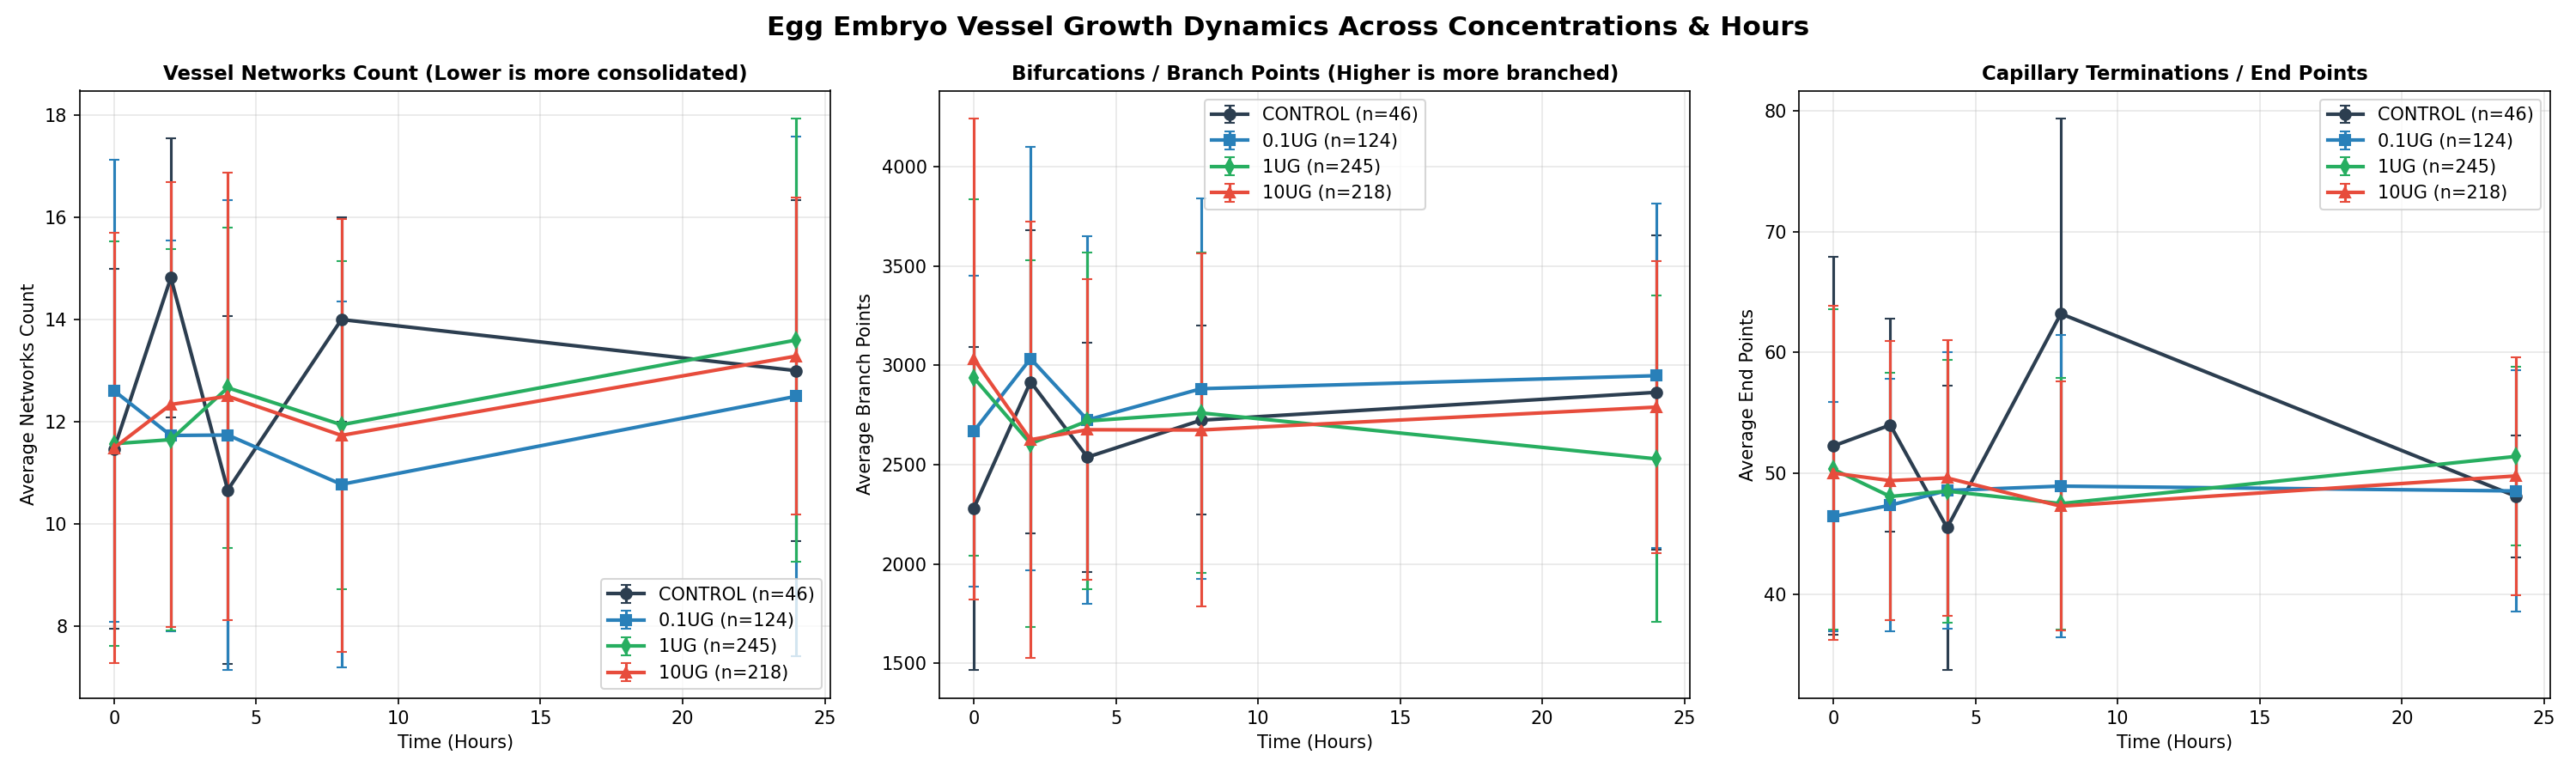
\includegraphics[width=\textwidth]{images/vessel_growth_plots.png}
\caption{Egg Embryo Vessel Growth Dynamics (Networks, Branches, and Endpoints) across Concentrations and Time Points.}
\label{fig:egg_embryo_curves}
\end{figure}

\subsection{Kinetics of Vascular Consolidation}
The count of distinct vessel networks serves as a proxy for vascular continuity and consolidation. In this metric, a lower number signifies that disjointed vascular segments have successfully met and fused (anastomosis) to form a unified, continuous circulatory web, whereas a higher count represents fragmentation.

As shown in Figure~\ref{fig:egg_embryo_curves} (left panel), the Control group displays high volatility, peaking at 2h ($14.82 \pm 2.72$ networks) and 8h ($14.00 \pm 2.00$ networks). This indicates unstable, unguided sprouting dynamics in the absence of chemical intervention. Conversely, the 0.1\,$\mu$g group shows rapid consolidation, with network counts dropping to $10.78 \pm 3.58$ at 8h. The 1\,$\mu$g group demonstrates a highly stable, regulated progression, avoiding the erratic spikes of the Control group, suggesting structured vascular development.

\subsection{Kinetics of Branching Complexity}
Vessel branching (bifurcation count) indicates angiogenic sprouting activity and network density. A higher branch point count represents a more complex, dense capillary network.

As visualized in the middle panel of Figure~\ref{fig:egg_embryo_curves}, the low-dose group (0.1\,$\mu$g) acts as a strong stimulant, maintaining the highest average branching complexity over time (peaking at $3033.93 \pm 1065.80$ branch points at 2h and sustaining $2948.00 \pm 866.08$ at 24h). In contrast, the higher doses (1\,$\mu$g and 10\,$\mu$g) show a downward trajectory after 0h, stabilizing around ~2500--2700 branch points. This indicates a pruning effect where higher concentrations regulate and organize the capillaries into a cleaner, more efficient, and mature layout rather than an over-congested, chaotic vascular bed.

\subsection{Capillary Loop Connection (Endpoints)}
Endpoints represent blind-ending capillary tips that are seeking vascular connection. As loop connection (anastomosis) occurs, endpoints merge to form closed-loop circuits, causing the endpoint count to drop.

The Control group displays a large accumulation of blind-ending, non-functional capillary tips at 8h ($63.20 \pm 16.17$ endpoints), indicating a failure of sprouts to close loops. In contrast, all three drug-treated groups maintain low, highly stable endpoint counts (~46--51) throughout the experiment. This proves that the drug treatment successfully coordinates vessel sprouts, ensuring they rapidly find other vessels to establish closed-loop circulation.

\section{Limitations of the Proposed Methodology}
While the quantitative and qualitative results are highly promising, a rigorous academic analysis requires an explicit acknowledgment of the methodology's current limitations.

The primary limitation involves the binarization thresholding step prior to skeletonization. We currently utilize a static threshold ($\tau = 0.5$). While highly effective for the confident predictions of the primary vessels, this static threshold can inadvertently break the continuity of ultra-thin capillaries whose predicted probabilities hover closely around $0.45 - 0.55$. When a continuous vessel is thresholded into a dashed line, the skeletonization algorithm falsely interprets each dash as a distinct network, artificially inflating the "Connected Networks Count" and introducing spurious "End Points." 

Future iterations of this pipeline must investigate adaptive, hysteresis-based thresholding algorithms (similar to the Canny edge detector logic) that track the probability ridge-lines to preserve the connectivity of low-confidence micro-capillaries prior to morphological thinning.
